\chapter{Valg av metode}
Dette kapitlet beskriver valget av metode for med tanke på forskningsdelen av prosjektet. En forskningsplan har blitt utformet i henhold til rammeverket utviklet av Oates \cite{oatesResearchingInformationSystems2013} i boken \textit{Researching Information Systems and Computing}. Her beskriver hun utviklingen av en forskningsplan og deler det inn i seks deler kalt \textit{The 6Ps of Research} (De 6 P-ene innenfor forsknings): \textit{Puropse} (Formål), \textit{Products} (Produkter), \textit{Process} (Prosess), \textit{Participants} (Deltakere), \textit{Paradigm} (Paradigme) og \textit{Presentation} (Presentasjon). Paradigme vil ikke bli diskutert da det ikke er nødvendig ettersom at dette i hovedsak er et systemutviklingsprosjekt.

\section{Formål}
Her beskrives bakgrunnen for prosjektet, samt tidligere forskning innenfor samme felt. Det forklares hva som skiller vår forskning fra eksisterende forskning, og til slutt vil forskningsspørsmålene for prosjektet bli presentert.
\newline
\newline
\noindent
Bakgrunnen for oppgaven blir beskrevet i kapittel \ref{bakgrunn} \nameref{bakgrunn} og formålet blir beskrevet i underkapittel \ref{sec:mal-for-oppgaven} \nameref{sec:mal-for-oppgaven}. For å oppsummere er målet med oppgaven å utvikle en applikasjon som kan ta over for dagens løsning med penn og papir i forbindelse med registrering av informasjon under en oppsynstur. Applikasjonen som skal utvikles må både dekke dagens behov, men også tilby en løsning for blind interaksjon med en hånd mens brukeren ser gjennom en kikkert og gjøre det mulig for gjetere og bønder å dele informasjon innad i et beitelag. Tidligere forskning og løsninger innfor samme område inkluderer applikasjonen Beitesnap \cite{BeitesnapRevolusjonerendeVerktoy} av Fant AS fra 2017, et verktøy laget for å registrere observasjoner av husdyr på beitet. Et annet eksempel på tidligere arbeid er masteroppgaven \textit{Effektivisering av manuell oppfølging av sau på utmarksbeite} hvor Dysthe og Kjerstad \cite{dystheEffektiviseringAvManuell2018} utforsker en løsning for registrering av saueflokker i forbindelse med oppsynsturer. Det som skiller denne løsningen fra tidligere arbeid er at den vil gi brukerne muligheten til å registrere saueflokker blindt med en hånd mens brukeren ser gjennom en kikkert. Dette er nødvendig da sauflokkene på utmarksbeitet ofte er så langt unna at man ikke klarer å registrere nødvendig informasjon uten å ta i bruk kikkert. Løsningen vil også være kryssplattform og fungere på mobile enheter som kjører både iOS og Android, noe som ble forsøkt av Dysthe og Kjerstad \cite{dystheEffektiviseringAvManuell2018} i 2018, men ble ikke fullført.
\newline
\newline
\noindent
I løpet av prosjektet vil det utvikles en fullverdig, fungerende versjon av en applikasjon som kan kjøre på både iOS og Android. Applikasjonen skal deretter brukertestes for å finne potensielle svakheter i designet. Ved å gjøre dette er det et ønske å svare på følgende forskningsspørsmål:

\begin{itemize}
    \item \textbf{F1: Hvordan utvikle et digitalt verktøy for å bistå sauebønder, beitelag og gjetere på oppsynstur slik at arbeidet med manuell registrering blir mer effektivt og raskere?}
    \item \textbf{F1.1: Kan man lage et system som erstatter dagens løsning med penn og papir, men fortsatt dekker alle brukerens behov?}
    \item \textbf{F1.2: Hvordan kan et digitalt system bistå sauebonde, beitelag og gjetere slik at de kan samhandle og dele informasjon om oppsynsturer med hverandre og norske myndigheter?}
    \item \textbf{F1.3: Hvordan utvikle et brukergrensesnitt som muliggjør registrering av sau uten å måtte se på mobilskjermen?}
    \item \textbf{F1.4: Hvordan utvikle et brukergrensesnitt som muliggjør registrering av sau under alle værforhold?}
\end{itemize}

\section{Produkter}
Dette underkapitlet forklarer hvilke produkter som vil komme som et resultatet forskningsprosjektet.
\newline
\newline
\noindent
Hovedproduktet fra forskningen vil være en applikasjon som kan erstatte dagens løsning for registrering av informasjon om saueflokker på utmarksbeitet med penn og papir. Samtidig skal applikasjonen tilby utvidet funksjonalitet med tanke på informasjonsflyt og brukbarhet. Selv om hovedmålet med prosjektet er å utvikle en applikasjon, vil resultatene både fra fordypningsprosjktet og selve masteroppgaven være med på å bidra til økt kunnskap om både utvikling av brukergrensesnitt for blind bruk, samt utvikling av kryssplattform-applikasjoner for bruk i forbindelse med informasjonsregistrering hvor man ikke har tilgang til internett der GPS og kart spiller en hovedrolle.

\section{Prosess}
Underkapittelet om prosess beskriver planen for hvordan det er tenkt å gå fram med forskningen under prosjektet. Prosessen baserer seg på figur \ref{fig:research_process} hentet fra \textit{Researching Information Systems and Computing} \cite{oatesResearchingInformationSystems2013}.
\newline
\newline
\noindent
Arbeidet med prosjektet var motivert av ønsket om å lage en applikasjon, utviklet basert på eksisterende litteratur, løsninger og forskning som kunne være med og bidra til å redusere antall sauer som dør hvert år på utmarksbeitet, samt gjøre arbeidshverdagen til sauebonder og gjetere enklere. Prosjektet startet med et litteratursøk inn i eksisterende løsninger for denne typen applikasjoner. Det ble også gjort et grundig arbeid for å kartlegge brukerens behov, basert både på dagens løsning men også hva som kreves fra myndighetens side. Dette både for å hjelpe til med å forme forskningsspørsmål, mens også for å kunne danne et konseptuelt rammeverk for prosjektet. 
\begin{figure}[H]
\centering
\captionsetup{width=.8\linewidth}
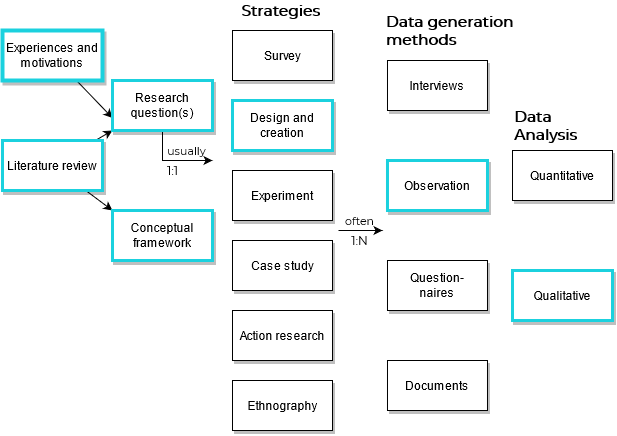
\includegraphics[scale=0.6]{Figurer/diagram/research_process.png}
\caption{Figuren viser den valgte veien for forskningsprosess markert med fargede bokser.}
\label{fig:research_process}
\source{\cite[~s.33]{oatesResearchingInformationSystems2013}}
\end{figure}

\noindent
Planen er å bruke \textit{Design og creation}-strategien for å implementere en applikasjon basert både på resultatene fra fordypningsprosjektet og litteratursøket. Når en ferdig førsteversjon av applikasjonen har blitt utviklet planlegger vi å brukerteste denne på fem ulike brukere. Her vil vi bruke \textit{Observation} som metode for å generere data fra brukertestene. Etter at testene er utført vil det bli gjort en kvalitativ analyse av dataene.

\section{Deltagere}
Dette kapitlet beskriver deltakerne i prosjektet og deres roller.
\newline
\newline
\noindent
Hoveddeltakerne i dette prosjektet vil være de som utfører selve prosjektet, altså Kimia Dadar Abtahi og Trym Vegard Gjelseth-Borgen. Personen som kommer til å veilede oss gjennom prosjektet, gi nyttig erfaringsbasert informasjon med tanke på oppsynsturer og som vil fungere som produkteier er Professor Svein-Olaf Hvasshovd. Det vil også være fem testdeltakere som deltar for å hjelpe til med brukertestene av applikasjonen. Data fra brukertestene og om testdeltakerne vil være anonymisert.

\section{Presentasjon}
Underkapitlet om presentasjon beskriver hvordan resultatene fra forskningsprosjektet vil bli presentert etter endt prosjekt.
\newline
\newline
\noindent
Resultatet av forskningen vil bli presentert i masteroppgaven. Resultatene vil også kunne være med på å utvikle en forbedret versjon av applikasjonen, hvis dette skulle være ønskelig etter prosjektets slutt.